%% Version 4.3.2, 25 August 2014
%
%%%%%%%%%%%%%%%%%%%%%%%%%%%%%%%%%%%%%%%%%%%%%%%%%%%%%%%%%%%%%%%%%%%%%%
% Template.tex --  LaTeX-based template for submissions to the 
% American Meteorological Society
%
% Template developed by Amy Hendrickson, 2013, TeXnology Inc., 
% amyh@texnology.com, http://www.texnology.com
% following earlier work by Brian Papa, American Meteorological Society
%
% Email questions to latex@ametsoc.org.
%
%%%%%%%%%%%%%%%%%%%%%%%%%%%%%%%%%%%%%%%%%%%%%%%%%%%%%%%%%%%%%%%%%%%%%
% PREAMBLE
%%%%%%%%%%%%%%%%%%%%%%%%%%%%%%%%%%%%%%%%%%%%%%%%%%%%%%%%%%%%%%%%%%%%%

%% Start with one of the following:
% DOUBLE-SPACED VERSION FOR SUBMISSION TO THE AMS
%\documentclass{ametsoc}

% TWO-COLUMN JOURNAL PAGE LAYOUT---FOR AUTHOR USE ONLY
 \documentclass[twocol]{ametsoc}

%%%%%%%%%%%%%%%%%%%%%%%%%%%%%%%%
%%% To be entered only if twocol option is used

\journal{mwr}

%  Please choose a journal abbreviation to use above from the following list:
% 
%   jamc     (Journal of Applied Meteorology and Climatology)
%   jtech     (Journal of Atmospheric and Oceanic Technology)
%   jhm      (Journal of Hydrometeorology)
%   jpo     (Journal of Physical Oceanography)
%   jas      (Journal of Atmospheric Sciences)	
%   jcli      (Journal of Climate)
%   mwr      (Monthly Weather Review)
%   wcas      (Weather, Climate, and Society)
%   waf       (Weather and Forecasting)
%   bams (Bulletin of the American Meteorological Society)
%   ei    (Earth Interactions)

%%%%%%%%%%%%%%%%%%%%%%%%%%%%%%%%
%Citations should be of the form ``author year''  not ``author, year''
\bibpunct{(}{)}{;}{a}{}{,}

%%%%%%%%%%%%%%%%%%%%%%%%%%%%%%%%

%%% To be entered by author:

%% May use \\ to break lines in title:

\title{Physics-dynamics coupling with element-based high-order Galerkin methods: quasi equal-area physics grid}

%%% Enter authors' names, as you see in this example:
%%% Use \correspondingauthor{} and \thanks{Current Affiliation:...}
%%% immediately following the appropriate author.
%%%
%%% Note that the \correspondingauthor{} command is NECESSARY.
%%% The \thanks{} commands are OPTIONAL.

    %\authors{Author One\correspondingauthor{Author One, 
    % American Meteorological Society, 
    % 45 Beacon St., Boston, MA 02108.}
% and Author Two\thanks{Current affiliation: American Meteorological Society, 
    % 45 Beacon St., Boston, MA 02108.}}

\authors{Adam R. Herrington\correspondingauthor{Peter H. Lauritzen, Climate and Global Dynamics, National Center for Atmospheric Research, 1850 Table Mesa Drive, Boulder, Colorado, USA.}}

%% Follow this form:
    % \affiliation{American Meteorological Society, 
    % Boston, Massachusetts.}

\affiliation{School of Marine and Atmospheric Sciences, Stony Brook University, State University of New York, Stony Brook, New York.}

%% Follow this form:
    %\email{latex@ametsoc.org}

\email{pel@ucar.edu}

%% If appropriate, add additional authors, different affiliations:
\extraauthor{Peter H. Lauritzen}
\extraaffil{Climate and Global Dynamics, National Center for Atmospheric Research, 1850 Table Mesa Drive, Boulder, Colorado, USA.}
\extraauthor{Mark A. Taylor}
\extraaffil{Sandia National Laboratories, Albuquerque, New Mexico, USA.}
\extraauthor{Paul A. Ullrich}
\extraaffil{Department of Land, Air and Water Resources, University of California, Davis, California, USA}
\extraauthor{Julio T. Bacmeister}
\extraaffil{Climate and Global Dynamics, National Center for Atmospheric Research, 1850 Table Mesa Drive, Boulder, Colorado, USA.}
\extraauthor{Steve Goldhaber}
\extraaffil{Climate and Global Dynamics, National Center for Atmospheric Research, 1850 Table Mesa Drive, Boulder, Colorado, USA.}

\extraauthor{Kevin A. Reed}
\extraaffil{School of Marine and Atmospheric Sciences, Stony Brook University, State University of New York, Stony Brook, New York.}

%% May repeat for a additional authors/affiliations:

%\extraauthor{}
%\extraaffil{}

%%%%%%%%%%%%%%%%%%%%%%%%%%%%%%%%%%%%%%%%%%%%%%%%%%%%%%%%%%%%%%%%%%%%%
% ABSTRACT
%
% Enter your abstract here
% Abstracts should not exceed 250 words in length!
%
% For BAMS authors only: If your article requires a Capsule Summary, please place the capsule text at the end of your abstract
% and identify it as the capsule. Example: This is the end of the abstract. (Capsule Summary) This is the capsule summary. 

\abstract{Enter the text of your abstract here.}

\begin{document}

%% Necessary!
\maketitle


%%%%%%%%%%%%%%%%%%%%%%%%%%%%%%%%%%%%%%%%%%%%%%%%%%%%%%%%%%%%%%%%%%%%%
% MAIN BODY OF PAPER
%%%%%%%%%%%%%%%%%%%%%%%%%%%%%%%%%%%%%%%%%%%%%%%%%%%%%%%%%%%%%%%%%%%%%
%

%% In all cases, if there is only one entry of this type within
%% the higher level heading, use the star form: 
%%
\begin{itemize}
\item We should compute TKE of tendencies and show that we ar removing scales with nc<2
\end{itemize}
\section{Introduction}
An increasing number of numerical methods publications in the atmospheric science literature concern transport, shallow-water, and three-dimensional models employing element-based high-order Galerkin discretizations such as finite-element and discontinuous Galerkin methods \citep[for an introduction to these methods see, e.g., ][]{Durran,NLL2011LNCSE}. Some global models based on Galerkin methods have reached a level of maturity for which they are being considered for next generation climate and weather models due to their inherent conservation properties, high-order accuracy (for smooth problems), high parallel efficiency, high processor efficiency, and geometric flexibility facilitating mesh-refinement applications. NCAR's Community Atmosphere Model \citep[CAM; ][]{CAM5} offers a dynamical core based on continuous Galerkin finite elements \citep{TF2010JCP}, referred to as CAM-SE \citep[CAM Spectral Elements; ][]{DetAl2012IJHPCA,TES2008JPCS,LetAl2017MWR}. CAM-SE is, in particular, being used for high resolution climate modeling \citep[e.g., ][]{JAME:JAME20125,BetAl2013JC,RetAl2015GRL} and static mesh-refinement applications \citep[e.g., ][]{FT2004MWR,ZetAl2014JC,ZetAl2014JCb,GetAl2014GMD,RHUZ2016}. Other examples of models based on high-order Galerkin methods that are being considered for `operational' weather-climate applications are \citet{Giraldo20083849}, \citet{NCT2009CF} and \citet{BSBDK2013TCFD}.

\begin{figure}[t]
\noindent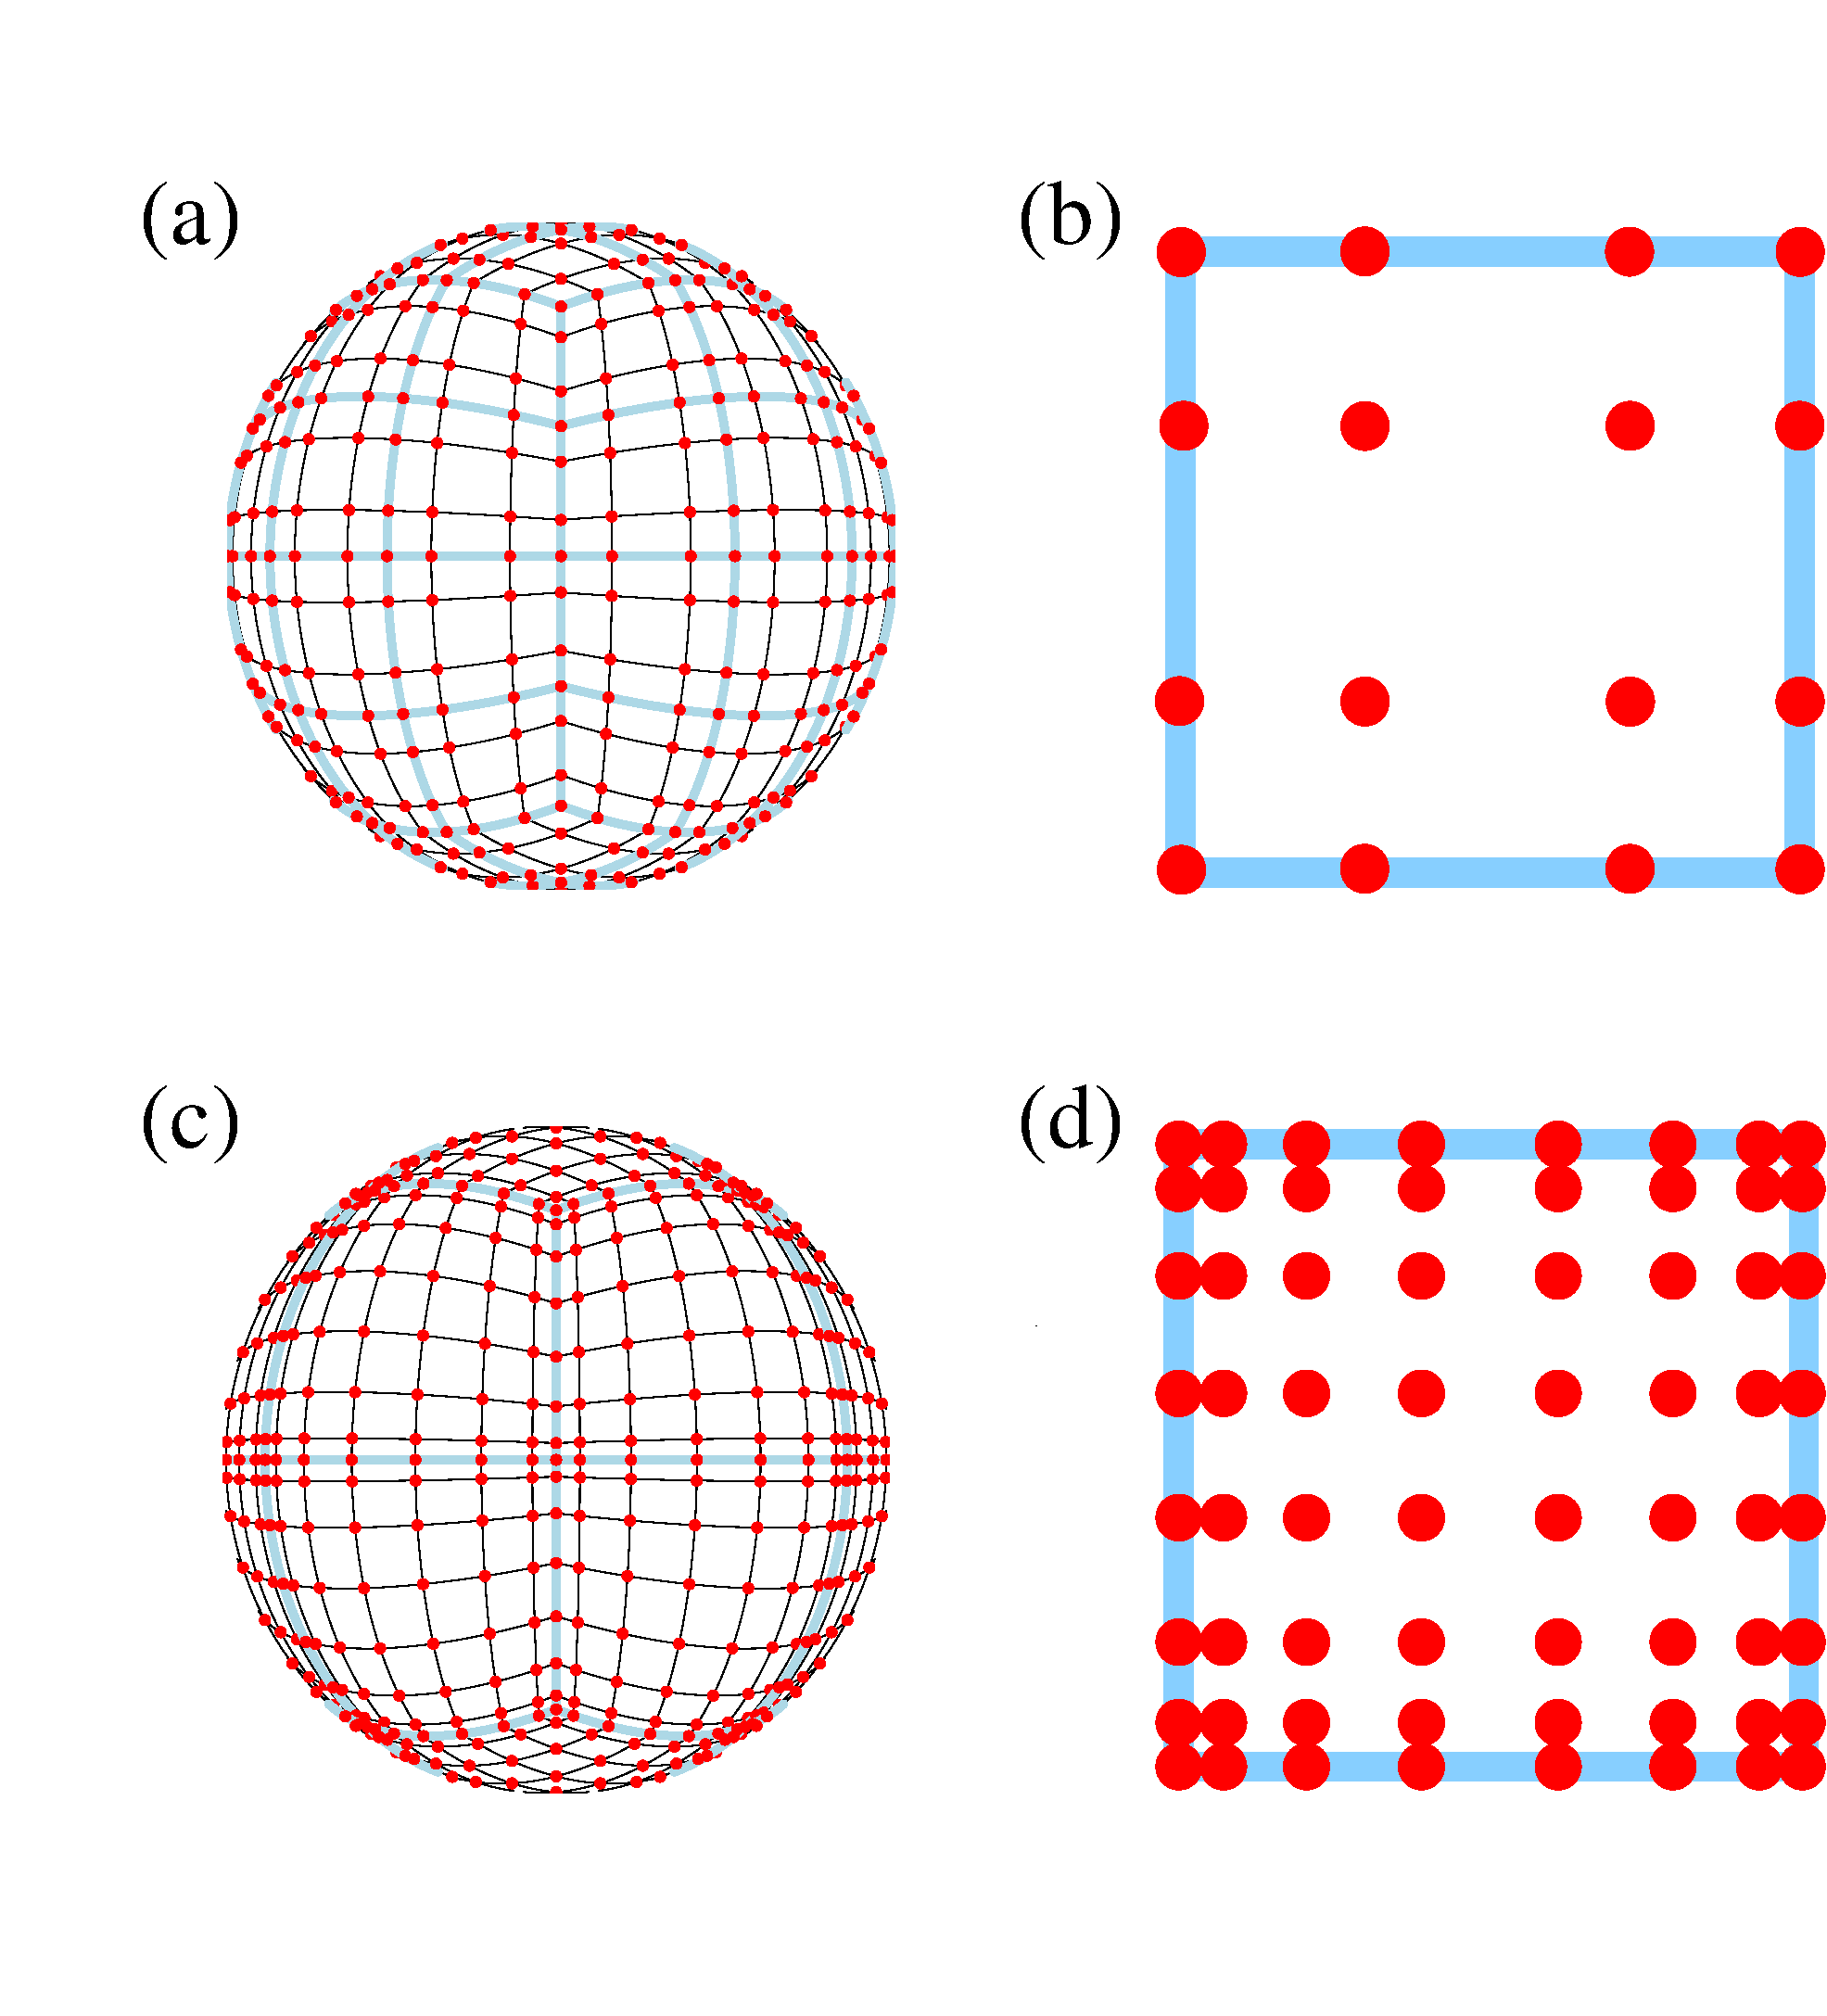
\includegraphics[width=19pc,angle=0]{figs/quadrature-fig/gll.pdf}\\
\caption{Example of CAM-SE GLL quadrature grids, marked with red filled circles, (a \& c) on the cubed-sphere and (b \& d) in an element. (a)-(b) and (c)-(d) use $4\times 4$ ($np=4$) and $8\times 8$ ($np=8$) GLL quadrature points in each element, respectively. (a) and (c) have the same average grid-spacing at the Equator (7.5$^\circ$) which is obtained by using (a) $4\times 4$ ($ne=4$) and (b) $2\times 2$ ($ne=2$) elements on each cubed-sphere face/panel, respectively. The element boundaries are marked with thick light blue lines. The grid configurations shown on (a) and (c) are referred to as $ne4np4$ and $ne2np8$, respectively.}
\label{fig:gll-grids}
\end{figure}

Traditionally the state of the atmosphere passed to the sub-grid-scale parameterizations (also referred to as {\em{physics}}) for models based on finite-volume and finite-difference methods has been the cell-averaged state in each control volume and the grid-point value, respectively. For the regular latitude-longitude, cubed-sphere and icosahedral grids the distance between the grid-points is gradually varying for finite-volume/finite-difference discretizations. If the same physics-dynamics coupling paradigm is applied to high-order element-based Galerkin methods, the state of the atmosphere passed to physics would be evaluated at the quadrature points. In the case of CAM-SE these are the Gauss-Lobatto-Legendre (GLL) quadrature points. Having the physics and dynamics grids coincide is obviously convenient since no interpolation is needed (which could disrupt conservation properties) and the number of degrees of freedom on both grids is exactly the same. A unique aspect of the high-order quadrature rules is that the nodes within an element are not equally spaced. For example, Figure \ref{fig:gll-grids} shows GLL points on an individual element of a cubed-sphere grid for degree 3 ($np=4$ quadrature points) and degree 7 ($np=8$ quadrature points) Lagrange polynomial basis in CAM-SE. Both grids have the same average resolution on the sphere (due to different number of elements), however, the higher the order of the quadrature rule the less equi-distant are the quadrature points. GLL quadrature points cluster near the edges and, in particular, the corners of the elements.

\begin{figure}[t]
\noindent\includegraphics[width=19pc,angle=0]{figs/se_gll_cv_grid.eps}\\
\caption{An example of control volumes constructed around GLL quadrature points (NE4NP4) so that the spherical area of the control volumes exactly match the quadrature weight multiplied by the metric factor.}
\label{fig:cv-grids}
\end{figure}

\begin{figure}[t]
\noindent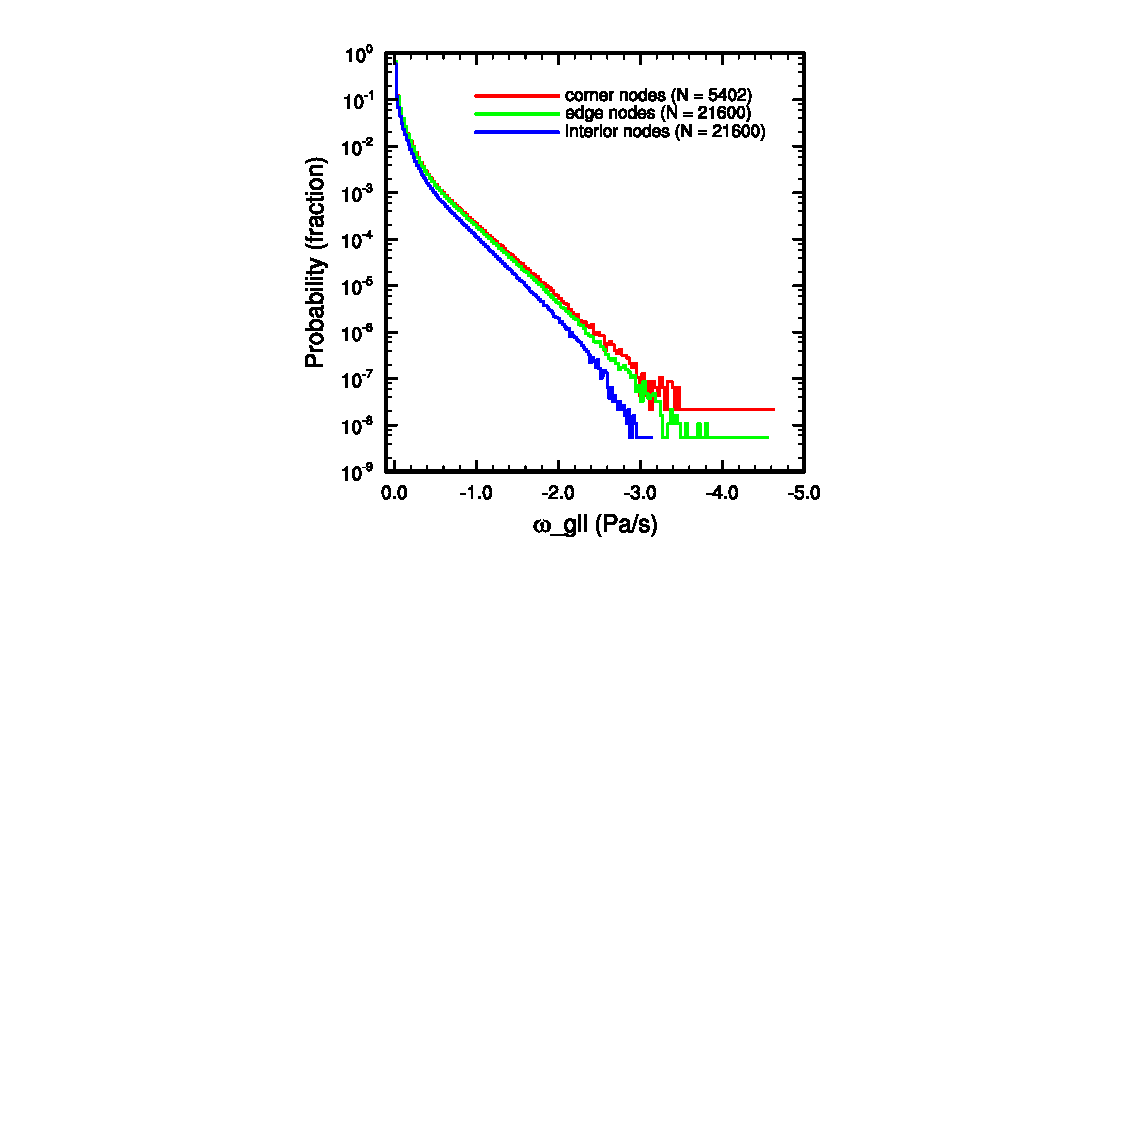
\includegraphics[width=19pc,angle=0]{figs/pdf_omg_gll_1panel.pdf}\\
\caption{PDF of instantaneous $\omega$ (1 month) classifying the points into small, medium, and large volumes/GLL 
weights. Note the consistent higher $omega$ values for smaller areas compared to $\omega$ associated with larger volumes (which makes sense). The question is how parameterizations respond to that.}\label{fig:omega-se-volumes}
\end{figure}

Parameterizations use the state of the atmosphere from the dynamical core as the large-scale state for computing sub-grid-scale processes. For example, the dynamical core state defines the large-scale environment in a mass-flux based convection scheme. One may think of the dynamical core state as the average state of the atmosphere over a control volume as inherent to finite-volume methods. For finite-difference methods the point value is thought of as representative for the atmospheric state in the vicinity of the point value and one can usually associate a volume with the grid-point. Hence the physics grid (the grid on which the state of the atmosphere is evaluated and passed to physics) and the dynamics grid (the grid the dynamical core uses) coincide. If we apply this concept to GLL quadrature values then a volume associated with the quadrature point should be defined. An example of that is shown on Figure \ref{fig:cv-grids} where control volumes have been defined around the quadrature points so that the spherical area of the control volumes exactly match the Gaussian weight multiplied by the metric term (these weights are used for integrating the basis functions over the elements and can therefore, in this context, be interpreted as areas). [{\color{red}{Mark: could we be mathematically more rigorous? perhaps an appendix describing the iterative algorithm?}}] This grid is used in the NCAR CESM (Community Earth System Model) coupler for passing states between ocean, atmosphere and land-ice components since the current remapping method is finite-volume based and therefore requires control volumes {\footnote{it is noted that methods exist that do not require control volumes for conservative interpolation \citep{UT2015MWR}}}. Hence the components `see' an irregular atmospheric grid. Similarly, the parameterizations in the atmosphere `see' a state that is anisotropically sampled in space \citep[see Figure 1 and 5 in ][]{KetAl2008JGR}. The effect of this grid anisotropy can be seen in moist simulations, such as aqua-planet experiments \citep{MWO2016JAMES,MWO2016JAMES}. Figure \ref{fig:omega-se-volumes} show a PDF of instantaneous upward vertical velocity $\omega$ for one year of an aqua-planet experiment using CAM-SE. The vertical velocity is classified by GLL weights pertaining to nodes lying on element corners ('corner nodes'), nodes along the element edges ('edge nodes') and nodes within the interior of an element ('interior nodes'). Consistently, the magnitude of $\omega$ is larger for smaller grid cell areas, due to the ability of smaller grid cells areas to support tighter horizontal gradients. [{\color{red}{The question is then how will the physics respond to this?}}]

\begin{figure*}[t]
\noindent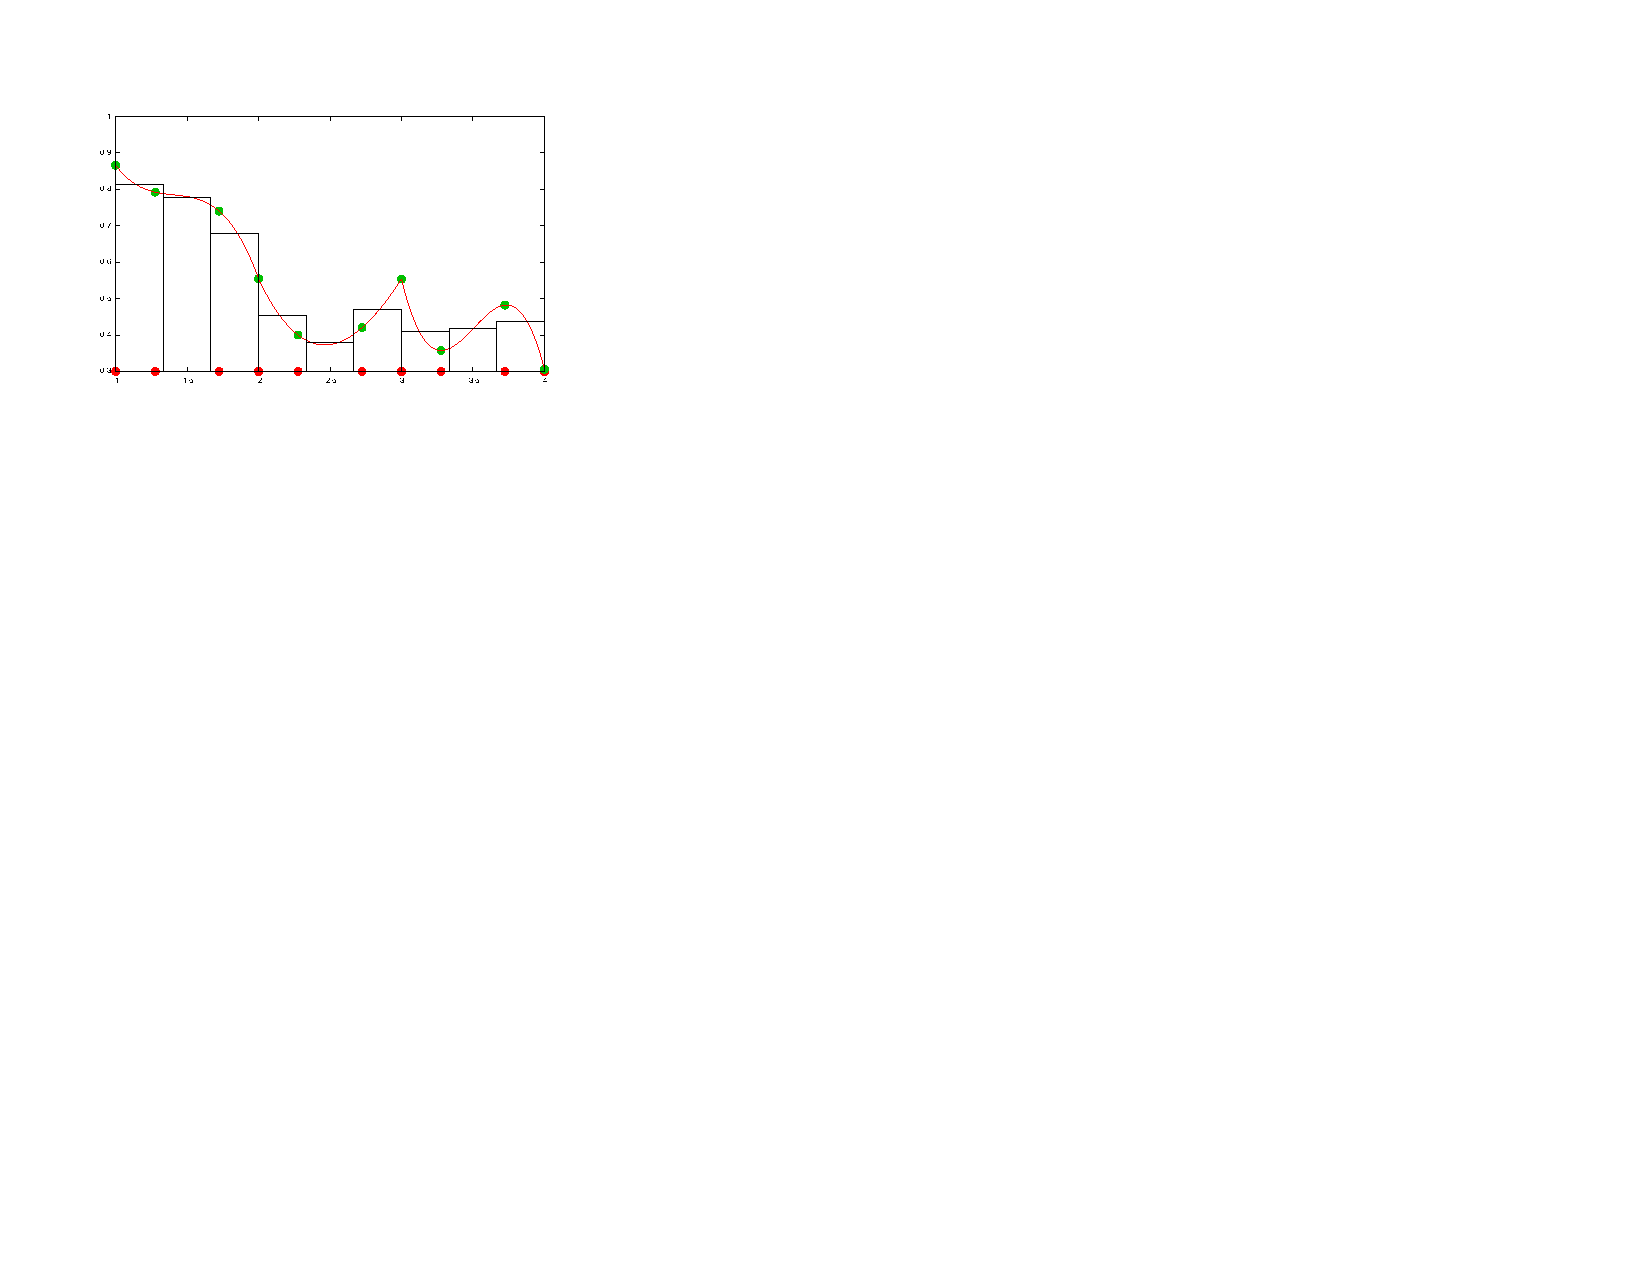
\includegraphics[width=38pc,angle=0]{figs/physgrid-1d_3x3.pdf}\\
\caption{A graphical illustration of the physics grid in one dimension. Three elements are shown and the filled red circles are the GLL quadrature points in each element. The red curve is the basis function representation of the field and the green filled circles are the quadrature point values. The physics grid divides each element into 3 equal-area control volumes. The histogram shows the average values over the physics grid control volumes resulting from integrating the basis functions over the respective control volumes.}
\label{fig:physgrid-1d}
\end{figure*}

The quadrature grid in high-order element-based Galerkin methods is defined to perform mathematical operations on the basis functions, e.g., computing gradients and integrals, rather than evaluating the state variables for physics-dynamics coupling. Within each element there is a high-order $C^{\infty}$ representation of state variables. One may argue that it would be more consistent to integrate the basis functions over quasi-equal area control volumes within each element and pass those control volume average values to physics rather than irregularly spaced quadrature point values. The relationship between the nodal values, the basis functions and the proposed control volumes is illustrated schematically in one-dimension in Figure \ref{fig:physgrid-1d}, and two dimension in Figure \ref{fig:grids}.

\begin{figure*}[t]
\noindent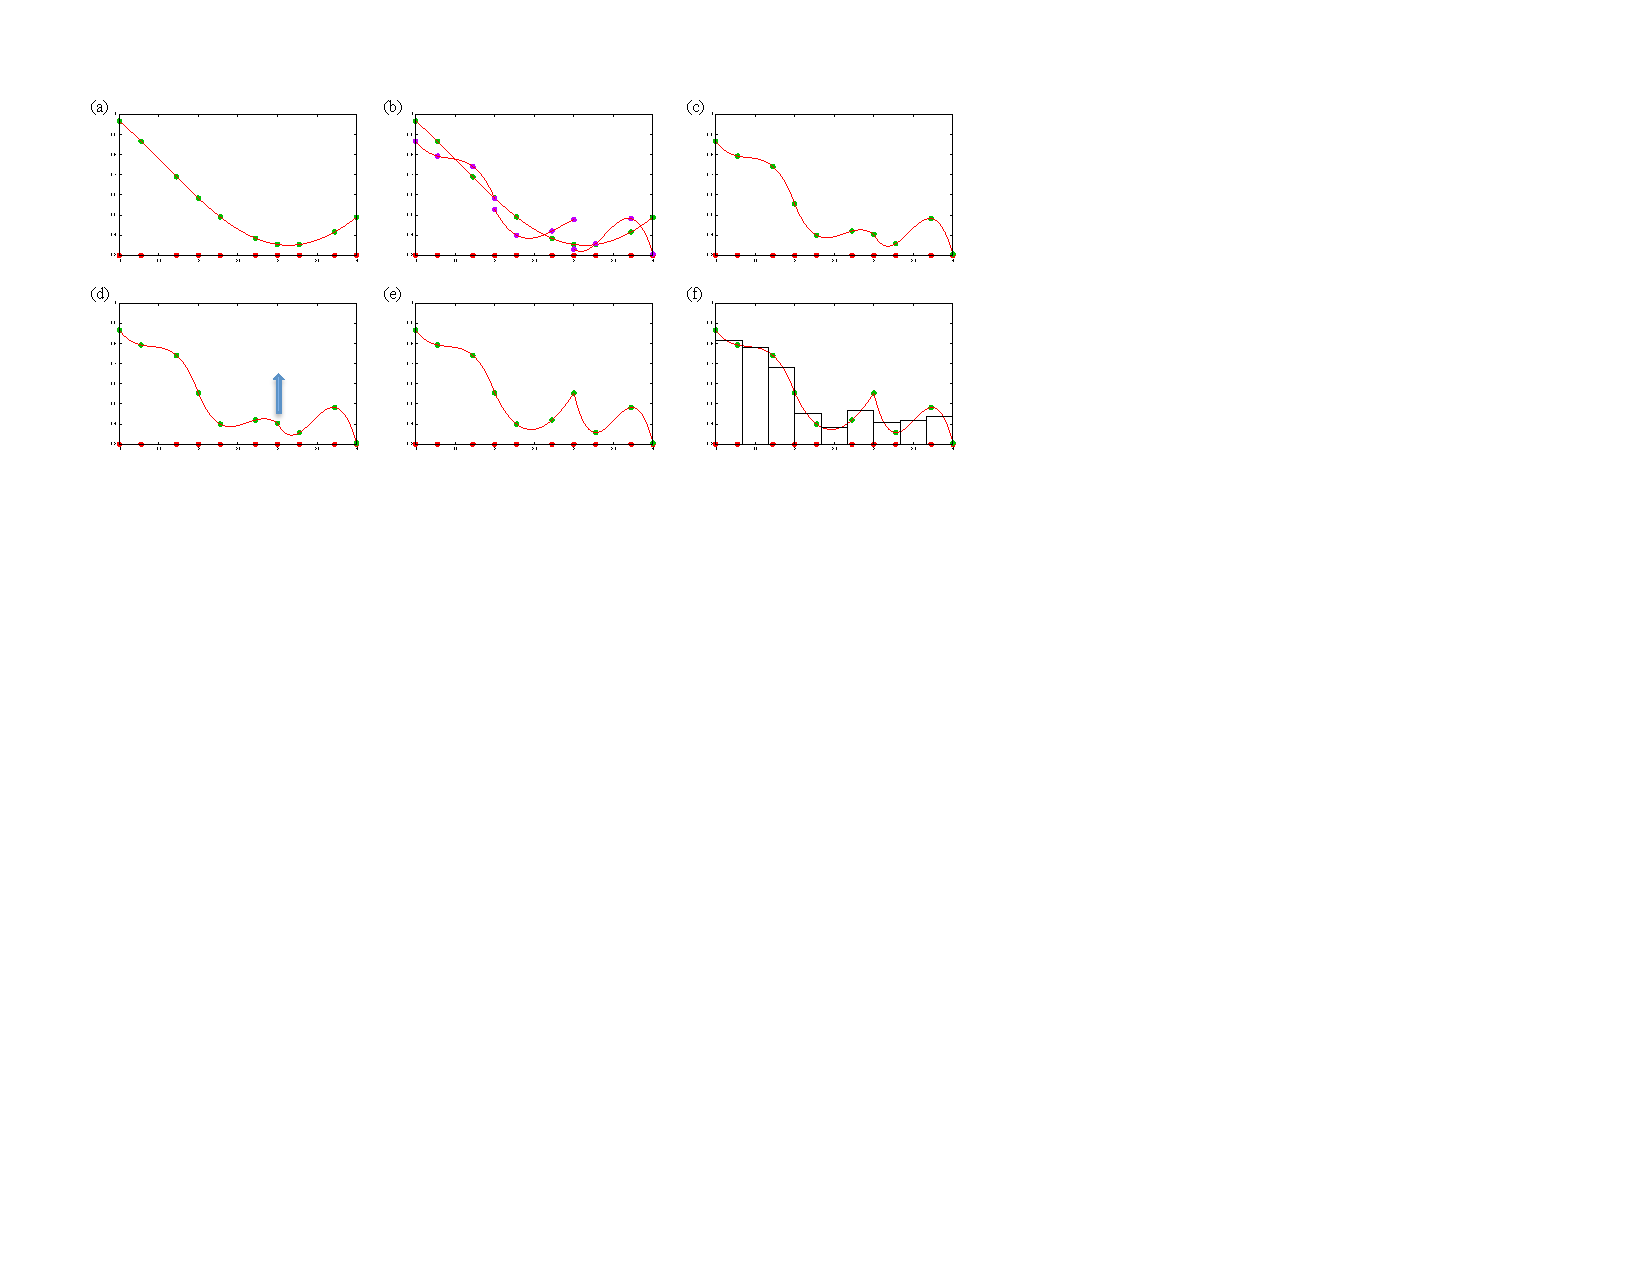
\includegraphics[width=38pc,angle=0]{figs/se-schematic.pdf}\\
\caption{A 1D schematic illustration on how CAM-SE advances the solution to the equations of motion in time. Consider 3 elements. The red filled circles are the GLL quadrature points in each element ($np=4$). Note that the quadrature points on the boundary are shared between elements. (a) Assume a degree 3 global Lagrange polynomial initial condition (red curve) which can be represented exactly by the degree 3 Lagrange basis in each element. (b) The solution to the equations of motion are advanced in time (one Runga-Kutta step) independently in each element leading to the quadrature values marked with filled purple circles. The Lagrange basis is shown with red curves connecting the purple circles. There are now two solutions, one from left and one from right, for the quadrature points at the element end points. In CAM-SE the values are averaged so that the solution is $C^0$. Note that the averaging changes the Lagrange polynomials throughout except at the internal quadrature points. (c) shows the solution after averaging. (d) Assume there is a grid-scale forcing that increases the quadrature value located at $x=3$. (e) The solution is now clearly $C^0$ at the element boundary at $x=3$. (f) Histogram shows the average values resulting in integrating the basis functions over the control volumes.}
\label{fig:se-schematic}
\end{figure*}

Integrating basis functions over control volumes may be beneficial in reducing the intrinsic oscillatory behavior of high-order basis functions within each element. Moreover, if there is a strong grid-scale forcing or oscillatory behavior near an element boundary, the solution will be least smooth near that element boundary. The element boundaries are least smooth since the boundary exchange of the continuous Galerkin method results in a degradation to $C^0$ along the element edges. This is illustrated in the context of CAM-SE on Figure \ref{fig:se-schematic}. In this case when integrating basis functions over control volumes a grid-cell average value is more representative of the values near the extrema at the element boundary than the quadrature point value.

%this should be included in the next paper (physres)
%When introducing a physics grid separate from the dynamics grid the question arises of what the resolution of the physics grid should be compared to the dynamics grid. For example, Figure \ref{fig:physgrid-1d} shows physics grids with the same, coarser and finer resolution than the GLL dynamics grid. From linear stability and accuracy analysis of numerical methods, it is a common result that the shortest resolvable wavelengths are not accurately represented. Similar arguments can be made from analyzing total kinetic energy spectra \citep{S2011LNCSE}. One may therefore argue that only believable scales should be passed to the physical parameterizations \citep{LH1997MWR}, i.e. a coarser resolution physics grid. This concept was investigated in a spectral transform model by \cite{W1999T}. On the other hand, computing physics tendencies on a higher-resolution grid compared to the dynamical core may provide a better sampling of the atmospheric state, somewhat similar to the super-parameterization \citep{G2001JAS,GRL:GRL14999,SA2007ASL} and sub-columns{\footnote{\citet{gmdd-8-5041-2015} in the context of CAM}} \citep{subcolumn,JGRD:JGRD10481} concepts. This approach was taken by \cite{M2009T} in the context of vertical refinement. \cite{W2014PTRSL} found improved forecast scores by increasing the grid-point space resolution compared to the resolution in wave-number space for the spectral transform model at ECMWF. 

%Alternatively, one could combine the two ideas and compute the state of the atmosphere on a coarser resolution grid and then use sub-columns or super-parameterization. One thereby passes believable scales to the sub-grid scale model and thereby assumes that a statistical sampling, in the case of sub-columns, or a simplified cloud-resolving model, in the case of super-parameterization, provides a more accurate sub-grid-scale tendency than sampling the Galerkin basis functions over the sub-grid-scale. [Discuss \cite{W2014PTRSL}: spectral truncation and physics (physical) grid (see page 10; conclusions)]




%Separating physics and dynamics grids has been investigated in the context of spectral transform models by \citet{TELA:TELA0009}, in which the separation was performed by truncation in wavenumber space. Parts of the physical parameterizations (microphysics) were separated in \citet{JGRD:JGRD50711} and vertical grid separation was investigated in \citet{TELA:TELA394}. In this study we run all of the parameterization on the physgrid.


%In the context of spectral transform model \citet{TELA:TELA0009} held the physics forcing scale fixed while refining the horizontal resolution of the dynamical core. In the context of microphysics \citet{JGRD:JGRD50711} did a scale separation and \citet{TELA:TELA394} separated the vertical grids. While \citet{LH1997MWR} and \citet{TELA:TELA0009} separated scales truncation of the the wave transform, we here separate scales through integrating basis functions over control volumes and , contrary to \citet{JGRD:JGRD50711}, all of the physical parameterization computations are performed on the physgrid. We focus on horizontal separation of scales here.

{\color{red}{It is the purpose of this paper to formulate the CAM-SE-physgrid version in which we separate physics and dynamics grids as illustrated in one dimension above. We show simulations from Held-Suarez .... CAM5 aquaplanet. ...}}



% \subsection*{subsection}
% text...
\section{Methods}
Here we focus on CAM-SE, however, in principle the methods apply to any element-based high-order Galerkin model. The physics grid in CAM-SE is defined by sub-dividing each element using equi-angular gnomonic coordinate lines to define the sides of the physics grid control volumes. Note that the element boundaries are defined by equi-angular gnomonic grid lines.  The notation $nc=3$ refers to the configuration where the elements are divided into $nc\times nc=3\times 3$ quasi equal-area physics grid cells (see Figure \ref{fig:grids}). Defining the physics grid by sub-diving elements makes it possible to use the same infrastructure as used for the quadrature point values thereby facilitating its implementation in CAM-SE. Here we make use of the $NE30NP4$, $NE30NP4NC2$, $NE30NP4NC3$, and $NE30NP4NC4$ grids that use GLL quadrature point physics grid (physics and dynamics grid coincide), coarser ($nc=2$), same ($nc=3$) and finer ($nc=4$) resolution quasi equal-area physics grids, respectively, compared to the GLL point resolution. In all configurations we use degree 3 Lagrange basis ($np=4$) and $ne\times ne=30\times 30$ elements on each cubed-sphere panel resulting in an average GLL quadrature point spacing at the Equator of $1^\circ$. Vertical grid spacing is the standard CAM5 configuration ($nlev=30$).

A consequence of separating physics and dynamics grids is that the atmospheric state must be mapped to the physics grid and the physics tendencies must be mapped back to the dynamics grid which is discussed in separate sections below. 
\subsection{Mapping state dynamics grid (GLL) to physics grid (physgrid)}
The dynamics state is defined on the GLL grid in terms of temperature $T^{(gll)}$, zonal wind component $u^{(gll)}$, meridional wind component $v^{(gll)}$, and dry pressure level thickness $\Delta p^{(gll)}$. In the mapping of the atmospheric state to the physics grid it is important that the following properties are met:
\begin{enumerate}
\item conservation of scalar quantities such as mass and thermal energy,\label{prop1}
\item for tracers; shape-preservation (monotonicity), i.e. the mapping method must not introduce new extrema in the interpolated field, in particular, negatives,\label{prop2}
\item consistency, i.e. the mapping preserves a constant,\label{prop3}
\item linear correlation preservation.
\end{enumerate}
Other properties that may be important, but not pursued here, is total energy conservation and axial angular momentum conservation. We argue that the most consistent method for mapping scalar state variables from the GLL grid to the physics grid is to integrate the Lagrange basis functions representation (used by the SE dynamical core) over the physics grid control volumes, i.e. integrate the basis function representation of $\Delta p^{(gll)}\times T^{(gll)}$ and $\Delta p^{(gll)}$ over the physics grid control volume \citep[see, e.g., ][]{LTOUNGK2017MWR,UT2015MWR}{\color{red}{add Appendix with details}}. Thermal energy and dry air mass is conserved and the mapping is consistent. For the wind, which is a vector, the latitude-longitude wind components are mapped by transforming to contra-variant wind components, evaluate the basis function representation thereof at the equi-angular center of the physics grid control volumes and then transform back to latitude-longitude coordinate system winds. 

The mapping of tracers is more problematic since the basis function representation is oscillatory although the shape-preserving filter guarantees shape-preservation at the GLL nodes \citep{GTS2014JCP}. To avoid this issue we use the CAM-SE-CSLAM version of CAM-SE where tracers are advected on the 3x3 physics grid. Note that in CAM-SE-CSLAM the dry mass internally predicted by CSLAM, $\Delta p^{(cslam)}$, is, by design, equal to $\Delta p^{(gll)}$ integrated over the CSLAM/physics grid control volume \citep{LTOUNGK2017MWR}. Since the tracer grid and physics grids are co-located and $\Delta p^{(physgrid)}=\Delta p^{(cslam)}$ then the  mass conservation, correlation preservation, consistency and shape-preservation constraints are trivially fulfilled.

\subsection{Mapping tendencies from physics grid (physgrid) to dynamics grid (GLL)}
The physics tendencies are computed on the finite-volume physics grid and are denoted $f_T^{(phys)}$,$f_u^{(phys)}$,$f_v^{(phys)}$, and $f_m^{(phys)}$. Note that dry air mass is not modified by physics and hence there is no tendency for dry mass,  $f_{\Delta p}\equiv 0$. Also, it is important to map tendencies and not state from the physics grid to GLL grid otherwise one will get spurious tendencies from mapping errors when the actual physics tendency is zero (unless a reversible map is used).

It is important that this process:
\begin{enumerate}
\item preserves a zero tendency,
\item for tracers; mass tendency is conserved,
\item for tracers; in each tracer grid cell the mass tendency from physics must not exceed tracer mass available in tracer grid cell (it is assumed that the physics tendency will not drive tracer mixing ratio negative on the physics grid),\label{item:phys2fvm_consistency}
\item linear correlation preservation,
\item consistency, i.e. the mapping preserves a constant.
\end{enumerate}
Other properties that may be important, but not pursued here, is total energy conservation (incl. components of total energy) and axial angular momentum conservation. Scalar variables are mapped from physics grid to GLL grid using a tensor-product Lagrange interpolation. The local coordinates on a cubed-sphere are discontinuous at the element edges so the interpolation requires special attention at the cube corners and edges. The details are provided in Appendix \ref{appendix}. Lagrange interpolation preserves a constant (including zero) and linear correlations. Tracer and physics grids are co-located so tracer mass, tracer shape, and tracer correlations are trivially preserved on the tracer grid; and the inconsistency in point \ref{item:phys2fvm_consistency} above will not appear. We do, however, need to map water tracers to the GLL grid to account for moist effects in the equations of motion. The CSLAM water tracer mixing ratios updated by physics tendencies are mapped to the GLL grid using the same tensor cubic interpolation as is used for temperature and velocity components. In between the calls to physics (i.e. in the dynamical core sub-stepping) the water tracers are advected on the GLL grid with the SE method.



\begin{itemize}
\item {\color{red}{mention why we are not doing cslam-like mapping; mention why we are not using Paul's algorithm}}
\item {\color{red}{in results section we might want to show some energy diagnostics and estimate PDC errors; must be run with $cp_{dry}$}}
\end{itemize}





% \section{Section title}
% \subsection{subsection one}
% text...
% \subsection{subsection two}
% \section{Section title}

%%%
\begin{figure}[t]
\noindent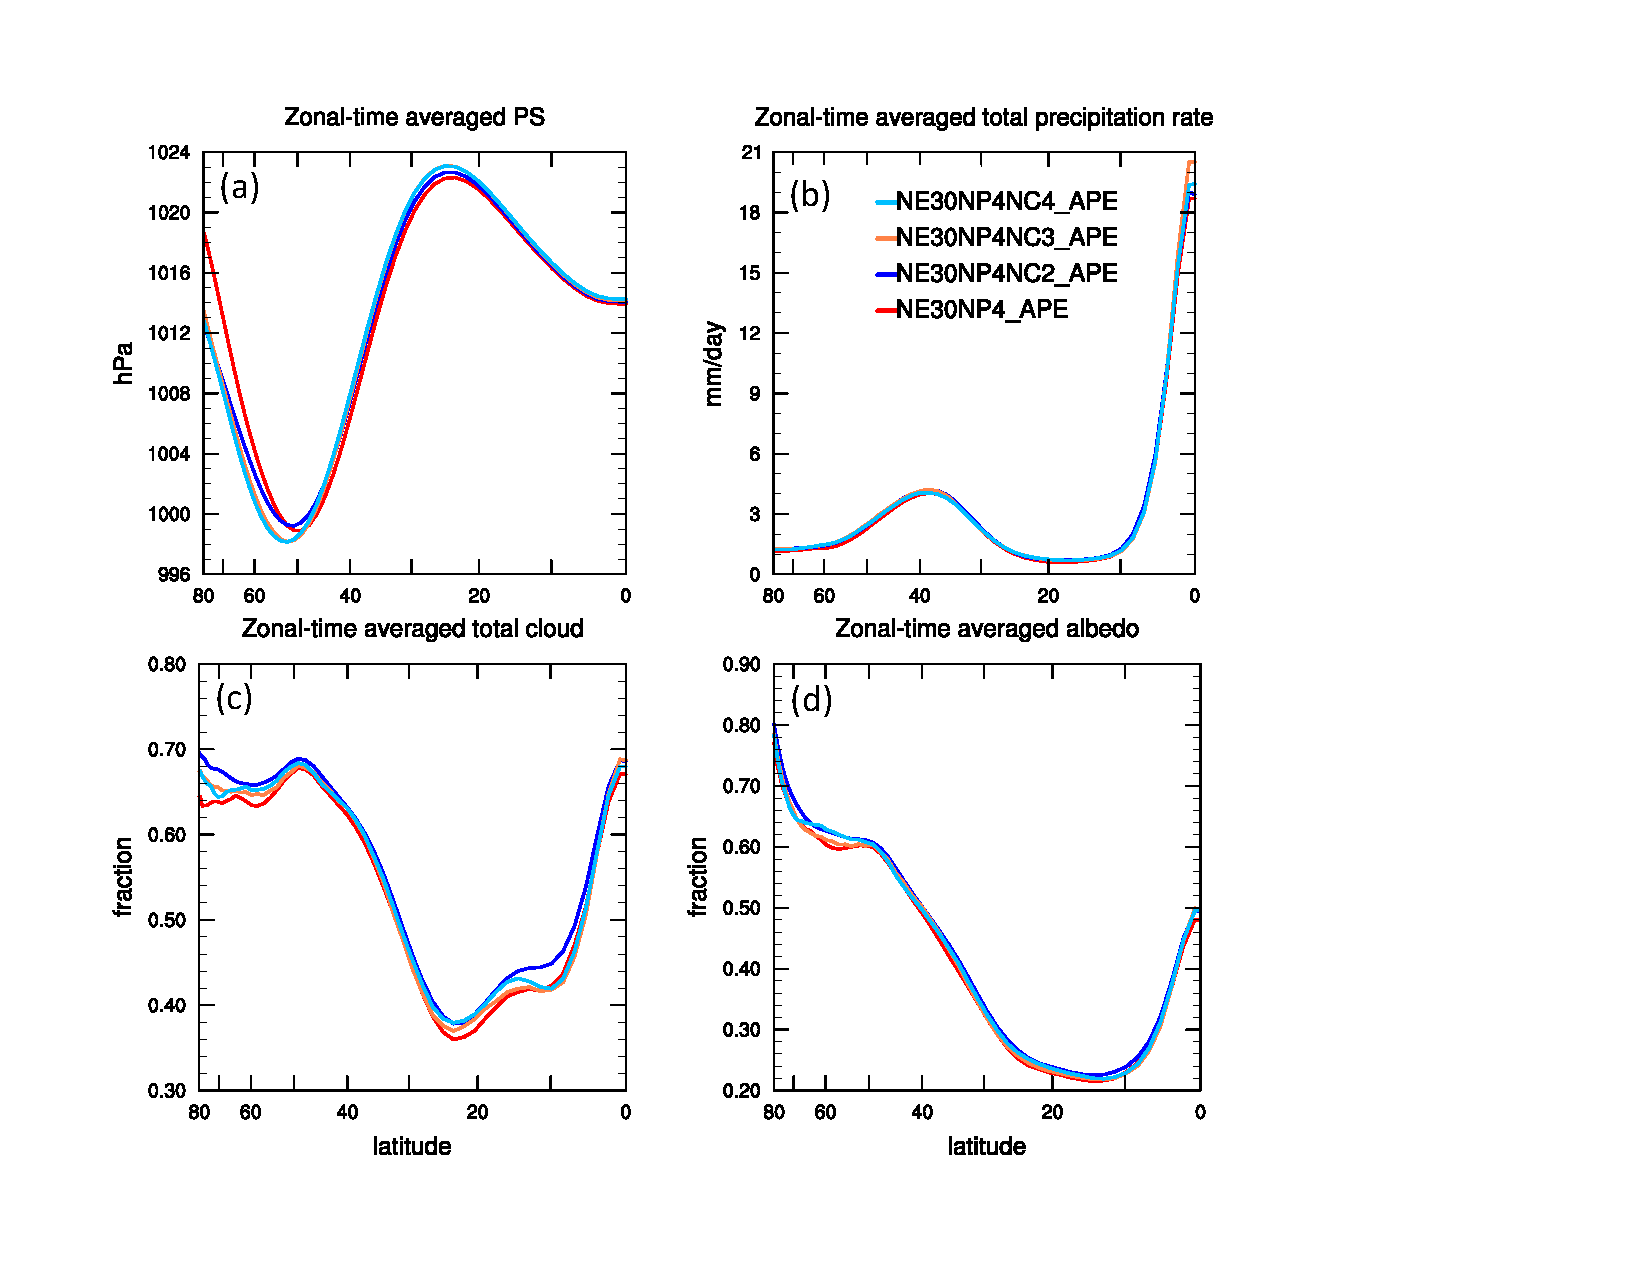
\includegraphics[width=19pc,angle=0]{figs/zonal_time_avg_2d_fields.pdf}\\
\caption{Zonal-time average (a) surface pressure $PS$, (b) total precipitation rate $PRECT$, (c) total cloud fraction $CLDTOT$, and (d) albedo as a function of latitude (from Equator to $80^\circ$N) for the different model configurations. The data has been averaged over a period of 30 months and mapped to a $1.5^\circ$$\times$$1.5^\circ$ regular latitude-longitude grid for analysis.}
\end{figure}

% \subsection{First secondary heading}

% \subsubsection{First tertiary heading}

% \paragraph{First quaternary heading}

%%%%%%%%%%%%%%%%%%%%%%%%%%%%%%%%%%%%%%%%%%%%%%%%%%%%%%%%%%%%%%%%%%%%%
% ACKNOWLEDGMENTS
%%%%%%%%%%%%%%%%%%%%%%%%%%%%%%%%%%%%%%%%%%%%%%%%%%%%%%%%%%%%%%%%%%%%%
%
\acknowledgments
NCAR is sponsored by the National Science Foundation (NSF).

%%%%%%%%%%%%%%%%%%%%%%%%%%%%%%%%%%%%%%%%%%%%%%%%%%%%%%%%%%%%%%%%%%%%%
% APPENDIXES
%%%%%%%%%%%%%%%%%%%%%%%%%%%%%%%%%%%%%%%%%%%%%%%%%%%%%%%%%%%%%%%%%%%%%
%
% Use \appendix if there is only one appendix.
%\appendix

% Use \appendix[A], \appendix}[B], if you have multiple appendixes.
%\appendix[A]

%% Appendix title is necessary! For appendix title:
%\appendixtitle{}

%%% Appendix section numbering (note, skip \section and begin with \subsection)
% \subsection{First primary heading}

% \subsubsection{First secondary heading}

% \paragraph{First tertiary heading}

%% Important!
%\appendcaption{<appendix letter and number>}{<caption>} 
%must be used for figures and tables in appendixes, e.g.,
%
%\begin{figure}
%\noindent\includegraphics[width=19pc,angle=0]{figure01.pdf}\\
%\appendcaption{A1}{Caption here.}
%\end{figure}
%
% All appendix figures/tables should be placed in order AFTER the main figures/tables, i.e., tables, appendix tables, figures, appendix figures.
%
%%%%%%%%%%%%%%%%%%%%%%%%%%%%%%%%%%%%%%%%%%%%%%%%%%%%%%%%%%%%%%%%%%%%%
% REFERENCES
%%%%%%%%%%%%%%%%%%%%%%%%%%%%%%%%%%%%%%%%%%%%%%%%%%%%%%%%%%%%%%%%%%%%%
% Make your BibTeX bibliography by using these commands:
\bibliographystyle{ametsoc2014}
\bibliography{bib}


%%%%%%%%%%%%%%%%%%%%%%%%%%%%%%%%%%%%%%%%%%%%%%%%%%%%%%%%%%%%%%%%%%%%%
% TABLES
%%%%%%%%%%%%%%%%%%%%%%%%%%%%%%%%%%%%%%%%%%%%%%%%%%%%%%%%%%%%%%%%%%%%%
%% Enter tables at the end of the document, before figures.
%%
%
%\begin{table}[t]
%\caption{This is a sample table caption and table layout.  Enter as many tables as
%  necessary at the end of your manuscript. Table from Lorenz (1963).}\label{t1}
%\begin{center}
%\begin{tabular}{ccccrrcrc}
%\hline\hline
%$N$ & $X$ & $Y$ & $Z$\\
%\hline
% 0000 & 0000 & 0010 & 0000 \\
% 0005 & 0004 & 0012 & 0000 \\
% 0010 & 0009 & 0020 & 0000 \\
% 0015 & 0016 & 0036 & 0002 \\
% 0020 & 0030 & 0066 & 0007 \\
% 0025 & 0054 & 0115 & 0024 \\
%\hline
%\end{tabular}
%\end{center}
%\end{table}

%%%%%%%%%%%%%%%%%%%%%%%%%%%%%%%%%%%%%%%%%%%%%%%%%%%%%%%%%%%%%%%%%%%%%
% FIGURES
%%%%%%%%%%%%%%%%%%%%%%%%%%%%%%%%%%%%%%%%%%%%%%%%%%%%%%%%%%%%%%%%%%%%%
%% Enter figures at the end of the document, after tables.
%%
%
%\begin{figure}[t]
%  \noindent\includegraphics[width=19pc,angle=0]{figure01.pdf}\\
%  \caption{Enter the caption for your figure here.  Repeat as
%  necessary for each of your figures. Figure from \protect\cite{Knutti2008}.}\label{f1}
%\end{figure}

\end{document}
